\beginsong{Circles}[wuw={Gwendolin Lee Zak, 1979, nach einem irischen Volkslied}, bo={204}, pfiii={94}, index={In days gone by}]

\markboth{\songtitle}{\songtitle}

\beginverse
\endverse

\centering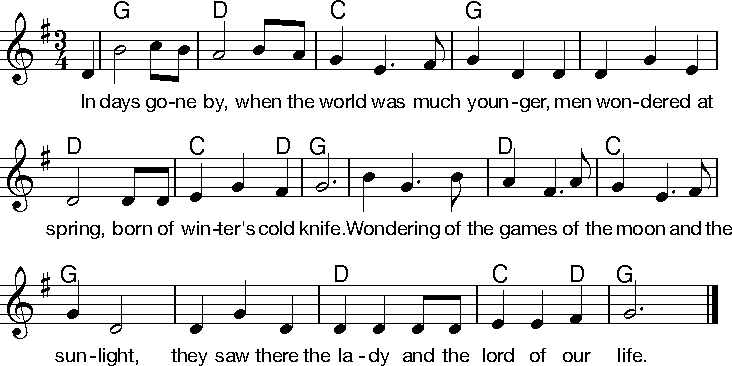
\includegraphics[width=1\textwidth]{Noten/Lied013.pdf}

\beginchorus
\[G]Round and a\[D]round and a\[C]round turns the \[G]good earth;
all things must \[D]change as the \[C]seasons \[D]go \[G]by.
We are the \[D]children of the \[C]Lord and the \[G]Lady,
whose mysteries we \[D]know but we \[C]never \[D]know \[C]why. \[G]
\endchorus 

\beginverse
\[G]In all lands the \[D]people have \[C]tried to the \[G]good earth,
ploughing and \[D]sawing as the \[C]seasons \[D]de\[G]clared,
waiting to \[D]reap of the \[C]rich golden \[G]harvest,
knowing their \[D]joy in the \[C]laughs that \[D]they \[G]shared.
\endverse
\renewcommand{\everychorus}{\textnote{\bf Refrain (wdh.)}}
\beginchorus
\endchorus

\beginverse
^Through Flandern and ^Wales and the ^green land of ^Ireland,
in the kingdoms of ^England and ^Scotland ^and ^Spain
circles grew ^up all a^long the wild ^coastline
and worked for the ^land with the ^sun and ^the ^rain.
\endverse

\beginchorus
\endchorus

\beginverse
^Circles for ^healing and ^working the ^weather,
circles for ^knowing the ^moon and ^the ^sun,
circles for ^thanking the ^Lord and the ^Lady,
circles for ^dancing the ^dance ne^ver ^done.
\endverse

\beginchorus
\endchorus

\endsong

\beginscripture{}
% nix g'fund'n
\endscripture

\begin{intersong}

\end{intersong}